%===================================== CHAP 5 =================================

\chapter{Verification}
\label{chp:verification}

The functionality of the extended CARP platform has been verified through
extensive testing, both through simulations and using the synthesised design
running on the Convey coprocessor.

\section{Tests}
\label{sec:test}

\subsection{Unit Tests}
\label{sec:unit-tests}

In addition to generating Verilog, Chisel is also capable of producing
cycle-accurate simulations of circuits in C++. The framework also provides tools
necessary for writing module-level unit tests that target these simulations. To
verify functionality and ensure interoperability with surrounding modules, tests
have been written for all modules implemented entirely in Chisel. These include
the InformationSender, Readout, SNNLAyer, Neuron, ReadoutSender and LUTWriter
modules. Modules that blackbox VHDL modules, such as the new CA module, can not
be simulated in this way, as the C++ simulator does not support mixed-language
simulation yet.

\subsection{Functional Tests}
\label{sec:functional-test}

To verify the integrity of the platform as a whole, Lundal wrote a series of
functional tests interacting with the hardware platform via the C API. These
have been updated and extended to ensure compatibility with changed
functionality. New tests have also been written to verify new functionality,
focusing especially on the interaction between the Readout and Cellular Automaton
modules.

Tests have been ran for multiple configurations of the system, including
for SBlock Matrices of different dimensions and Spiking Neural Networks with
different topologies.

\section{Example}
\label{sec:selfreg-example}

To showcase the functionality added to the system, the example organism in
\figurename~\ref{fig:example-development} has been created. It uses 10 cell
types and 19 development rules, and regulates its own growth through feedback
from the readout layer.

As shown in \figurename~\ref{fig:example-setup-ca}, the platform is configured
with an 8x8 matrix of cells. FeedbackCells are placed at coordinates (1, 1), (1,
5), (5, 1) and (5, 5), with the cells surrounding (1, 1) as output cells. The
developmental rules are created to have the organism grow in spirals around the
FeedbackCells. All cell types are associated with a LUT that sets their state to
1 regardless of the state of neighbors. Between each development step, two state
steps are performed. One to let the Readout module process the recently updated
states, and one to update the state of the FeedbackCells update their state
based on the output from the Readout module. As shown in
\figurename~\ref{fig:example-setup-readout}, the Readout module is configured
with a single neuron that will fire once it has received spikes along all input
edges. When all cells around the FeedbackCells are grown into, the Readout
module fires a spike. The development rules interpret this spike as a sign of
overpopulation and kills the cells directly above, below, left and right of the
FeedbackCells. The cells adjacent to these then die of starvation the next
development step.

This example shows how the Readout module can be used to classify the behavioral
dynamics of a cellular organism, and how that classification can be used to
regulate further growth and development.

\begin{figure}[ht]
  \centering
  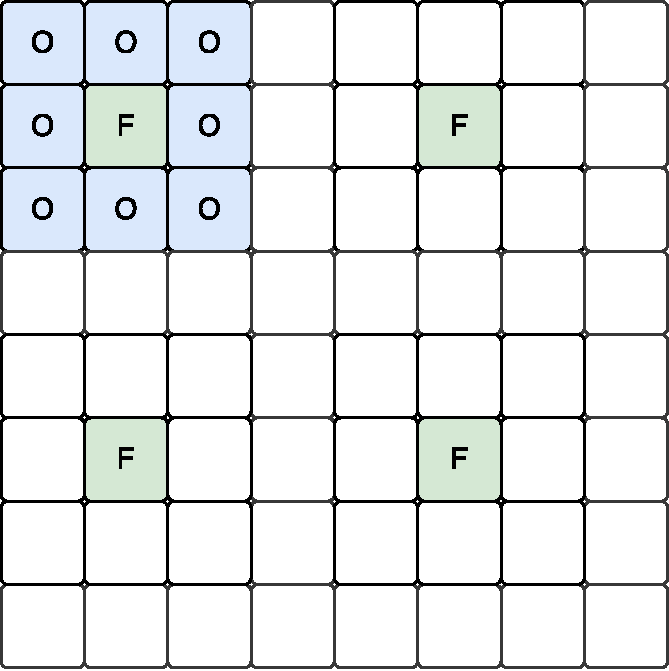
\includegraphics[width=0.4\linewidth]{fig/example-setup}
  \caption{
    CA configuration used in creating a self-regulating organism. Green cells
    are FeedbackCells, to which Readout output is routed, and blue cells are output
    cells, regular SBlocks whose output state is routed as input to the Readout
    module.
  }
  \label{fig:example-setup-ca}
\end{figure}

\begin{figure}[ht]
  \centering
  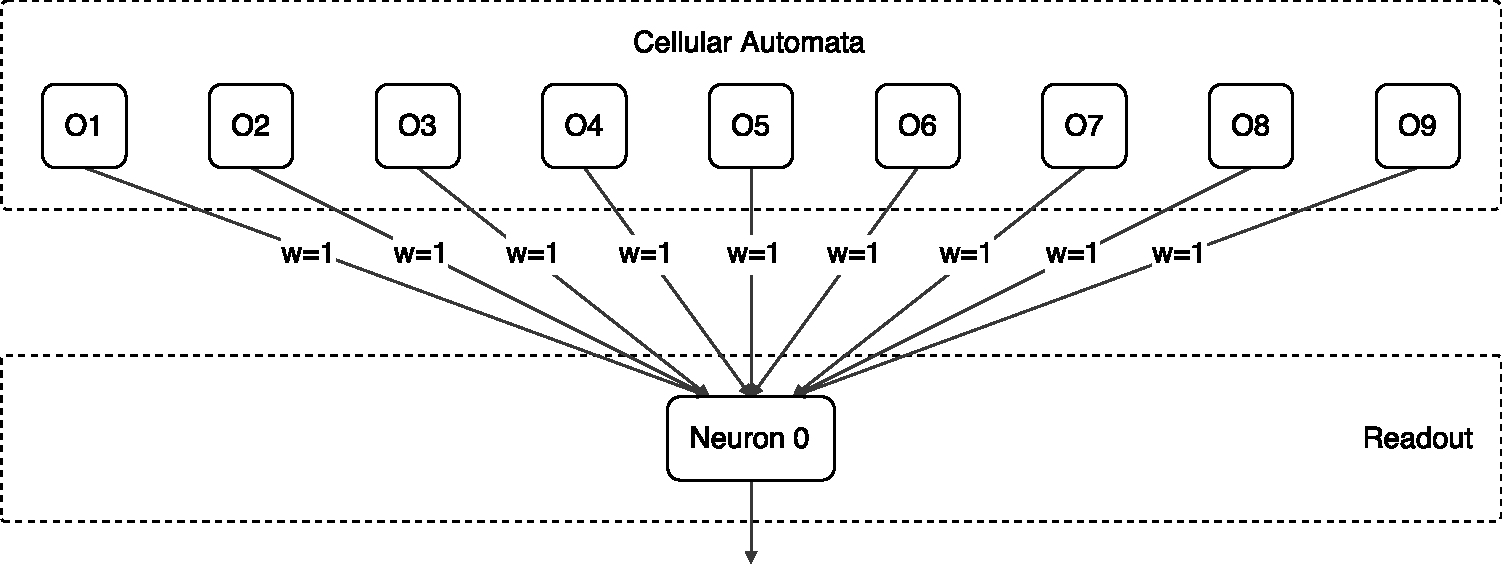
\includegraphics[width=\linewidth]{fig/example-readout}
  \caption{
    Configuration of the Readout module used in the example
    self-regulating organism
  }
  \label{fig:example-setup-readout}
\end{figure}

\begin{figure}[!ht]
  \centering
  \subfloat[Step 0]{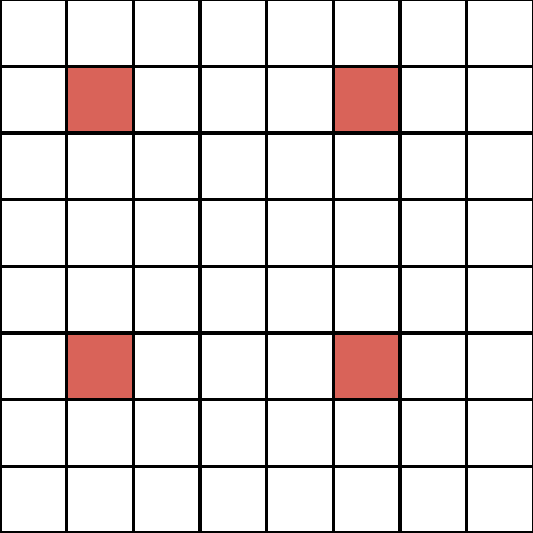
\includegraphics[width=0.30\linewidth]{fig/selfregulating/00}}
  \quad
  \subfloat[Step 1]{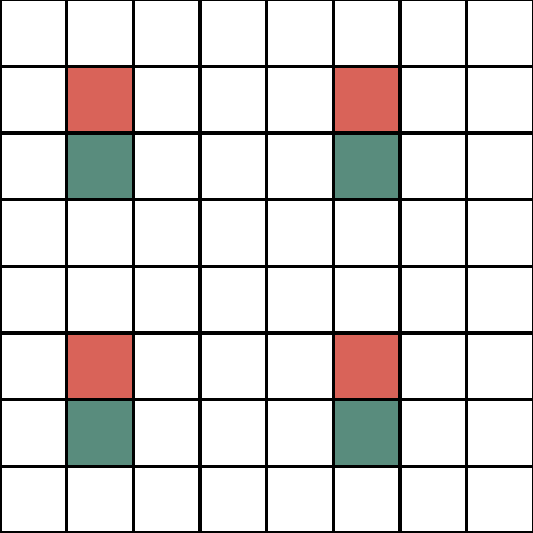
\includegraphics[width=0.30\linewidth]{fig/selfregulating/01}}
  \quad
  \subfloat[Step 2]{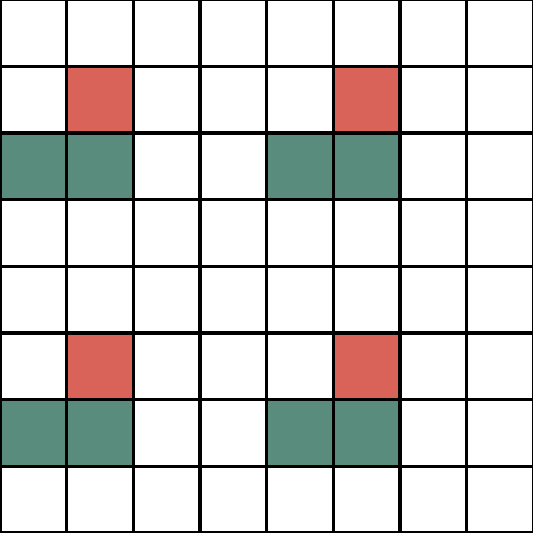
\includegraphics[width=0.30\linewidth]{fig/selfregulating/02}}
  \quad
  \subfloat[Step 3]{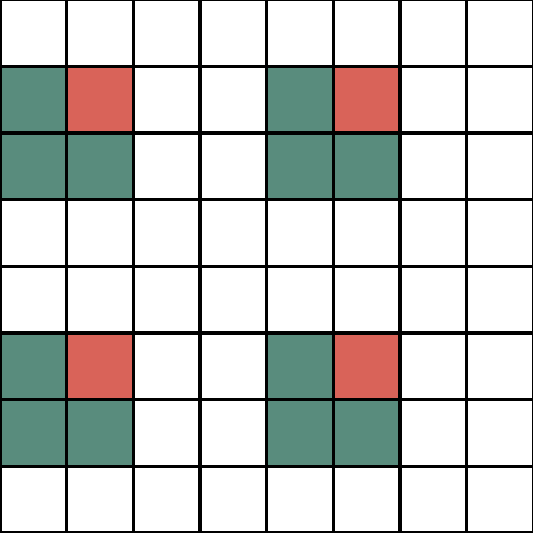
\includegraphics[width=0.30\linewidth]{fig/selfregulating/03}}
  \quad
  \subfloat[Step 4]{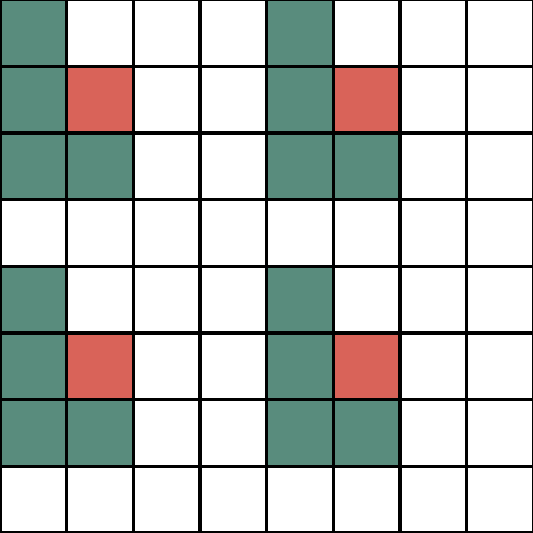
\includegraphics[width=0.30\linewidth]{fig/selfregulating/04}}
  \quad
  \subfloat[Step 5]{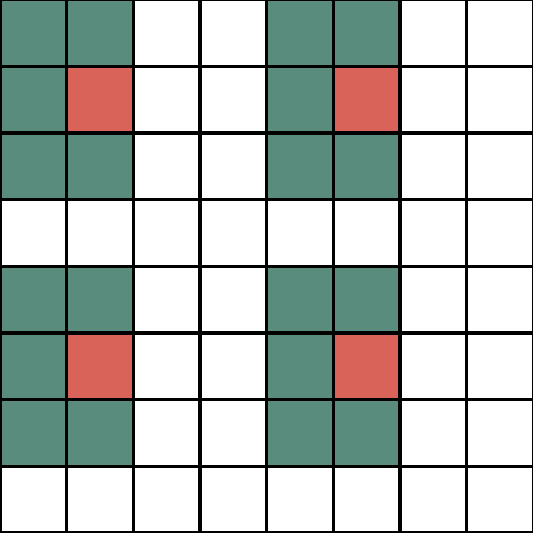
\includegraphics[width=0.30\linewidth]{fig/selfregulating/05}}
  \quad
  \subfloat[Step 6]{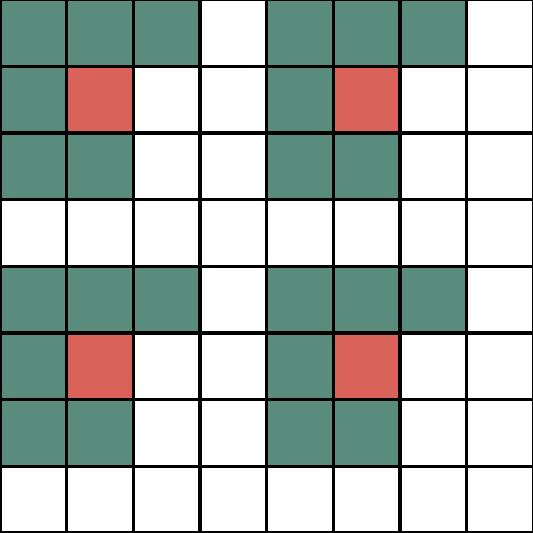
\includegraphics[width=0.30\linewidth]{fig/selfregulating/06}}
  \quad
  \subfloat[Step 7]{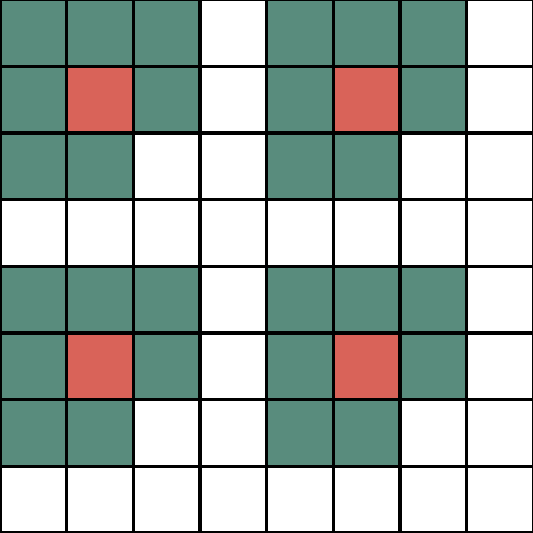
\includegraphics[width=0.30\linewidth]{fig/selfregulating/07}}
  \quad
  \subfloat[Step 8]{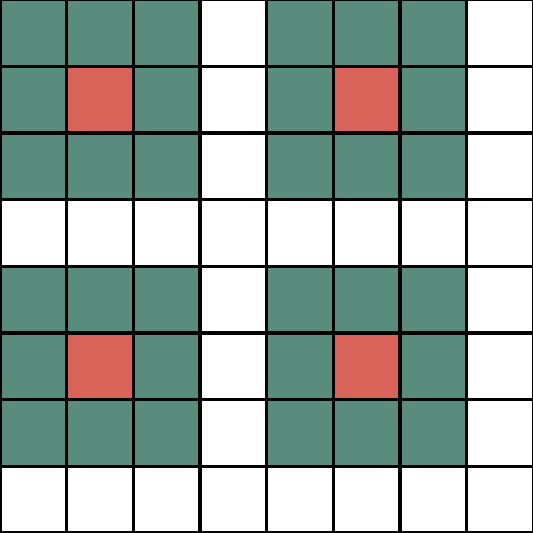
\includegraphics[width=0.30\linewidth]{fig/selfregulating/08}}
  \quad
  \subfloat[Step 9]{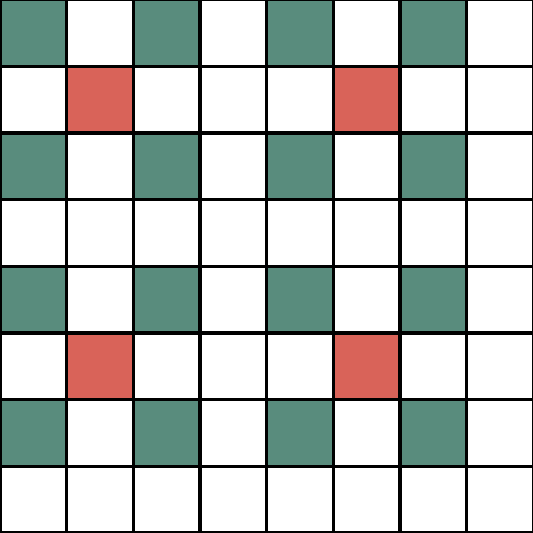
\includegraphics[width=0.30\linewidth]{fig/selfregulating/09}}
  \quad
  \subfloat[Step 10]{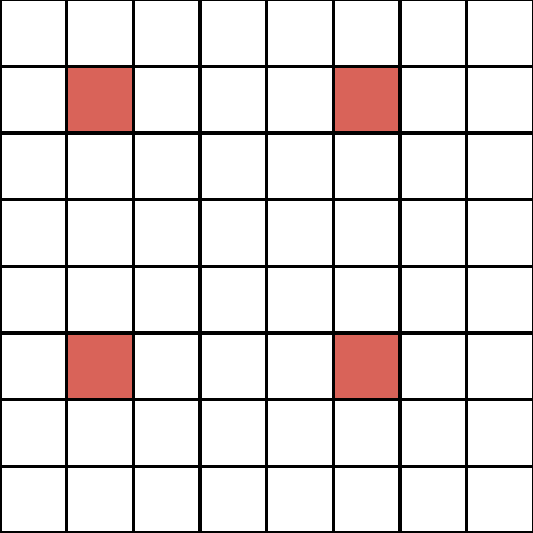
\includegraphics[width=0.30\linewidth]{fig/selfregulating/10}}
  \quad
  \subfloat[Step 11]{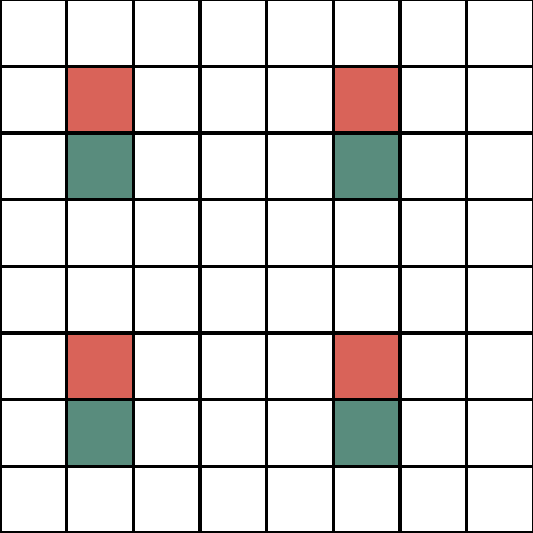
\includegraphics[width=0.30\linewidth]{fig/selfregulating/11}}
  \quad
\end{figure}

\begin{figure}[!ht]
  \centering
  \subfloat[Step 12]{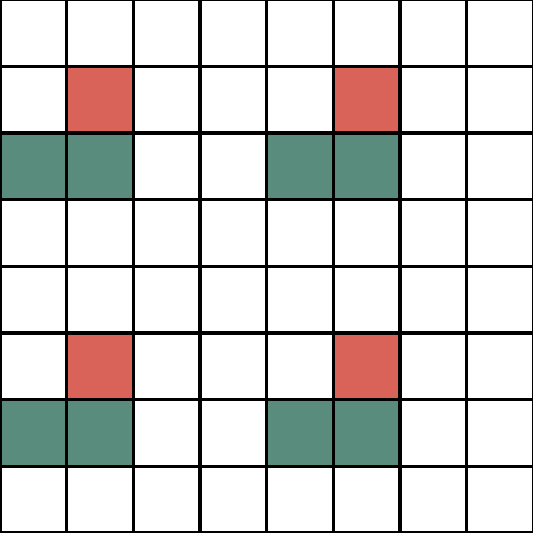
\includegraphics[width=0.30\linewidth]{fig/selfregulating/12}}
  \quad
  \subfloat[Step 13]{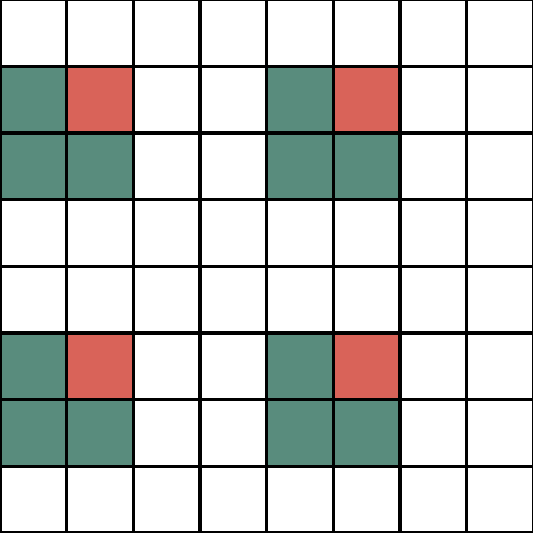
\includegraphics[width=0.30\linewidth]{fig/selfregulating/13}}
  \quad
  \subfloat[Step 14]{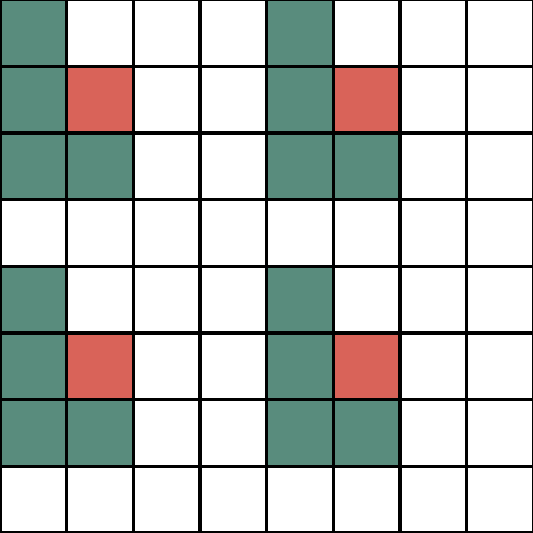
\includegraphics[width=0.30\linewidth]{fig/selfregulating/14}}
  \quad
  \subfloat[Step 15]{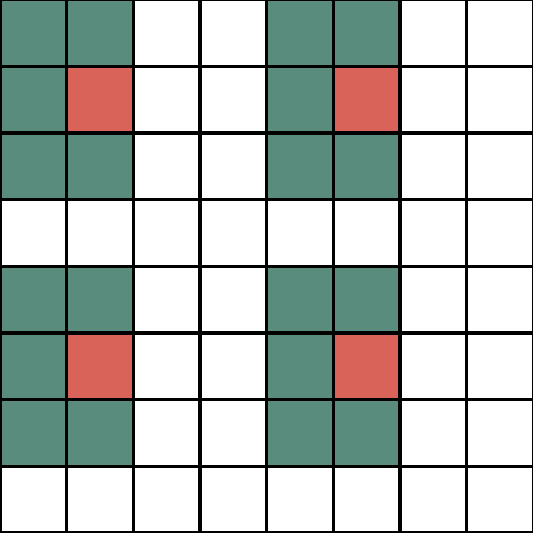
\includegraphics[width=0.30\linewidth]{fig/selfregulating/15}}
  \quad
  \subfloat[Step 16]{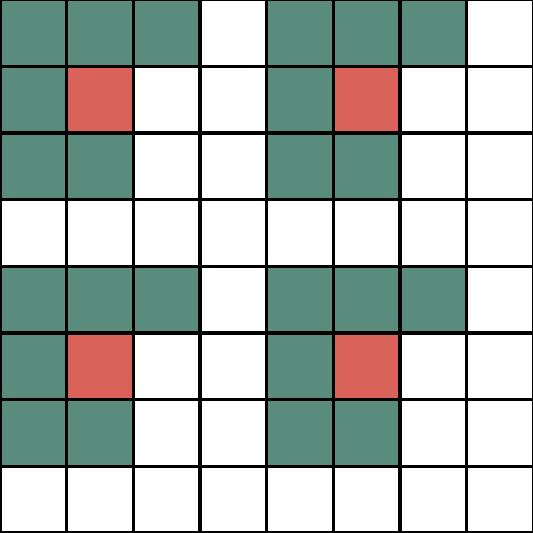
\includegraphics[width=0.30\linewidth]{fig/selfregulating/16}}
  \quad
  \subfloat[Step 17]{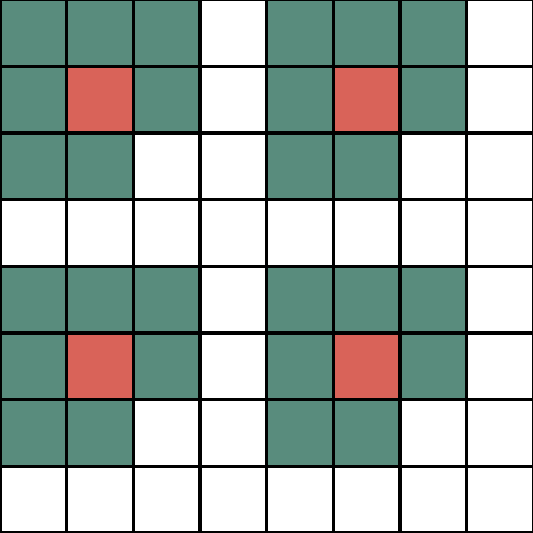
\includegraphics[width=0.30\linewidth]{fig/selfregulating/17}}
  \quad
  \subfloat[Step 18]{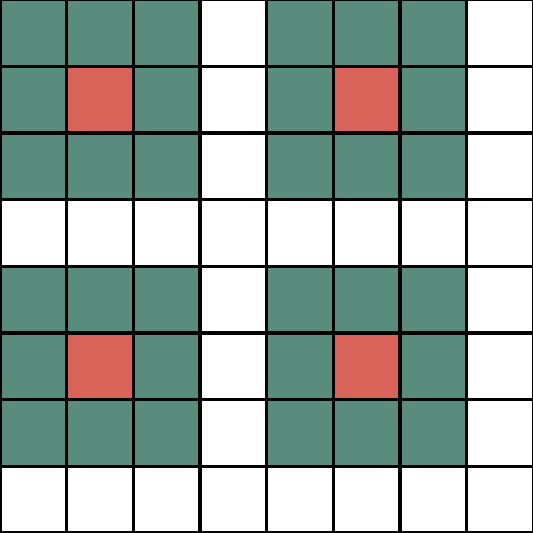
\includegraphics[width=0.30\linewidth]{fig/selfregulating/18}}
  \quad
  \subfloat[Step 19]{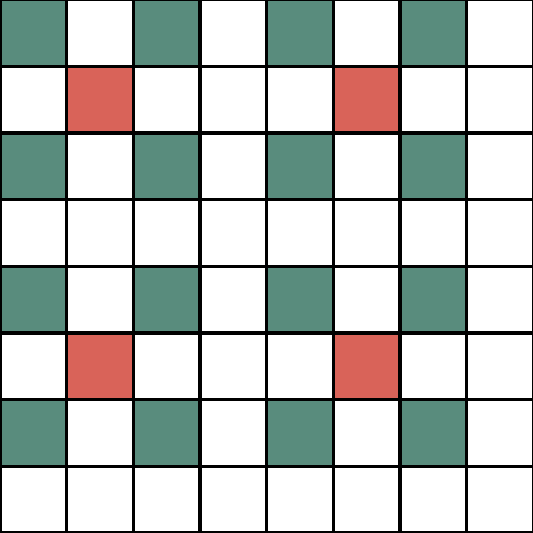
\includegraphics[width=0.30\linewidth]{fig/selfregulating/19}}
  \quad
  \subfloat[Step 20]{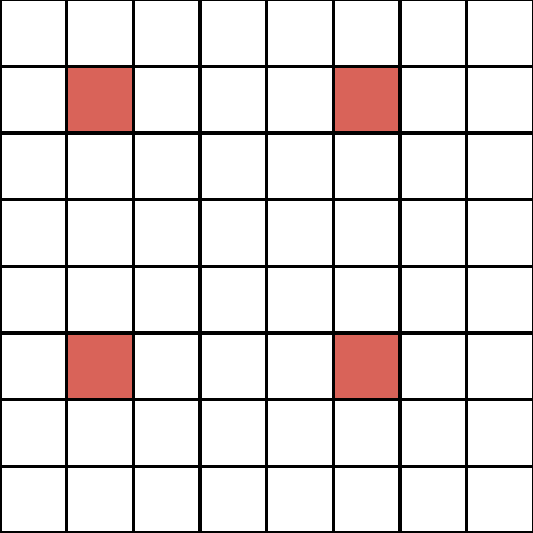
\includegraphics[width=0.30\linewidth]{fig/selfregulating/20}}
  \quad
  \caption{
    Development steps of a self-regulating cellular organism simulated on
    the CARP platform. At steps 9 and 19, the Readout module classifies the
    organism as overpopulated. The next development step, the organism reacts to
    this by killing off cells. The growth cycle subsequently restarts.
    \label{fig:example-development}
  }
\end{figure}
\cleardoublepage